\chapter{Communication}\label{cha:communication}

The goal of the project is to provide a teleoperated surgical system which makes the surgeon controlling the robot feel as if he was manipulating the end-effector directly. To achieve this, the time delay of the force between the end-effector and the controller should be unnoticeable. The targeted communication frequency of 1 kHz should result in a delay small enough to satisfy this need.\todo{What is the relation between sample rate and delay?}

\section{Communication between ROS and the sbRIO board in the current system}


In the former system setup the sbRIO board and the computer running ROS are communicating through an ethernet cable using the TCP/IP protocol. TCP/IP is a connection orientated protocol, which first establish the connection between two devices. After the connection has been established data can be send in both directions. TCP/IP is a reliable protocol which ensure that the data transmitted, will be received. When the data is send, the transmitter waits for an acknowledgment from the receiver that the data has been received. If the data has been corrupted or the acknowledgment is not send, the transmitter will retransmit the package again. If the case of no acknowledgment is happening, a timer is used to define when to retransmit the data again. The data will then be retransmitted a certain amount of times until an acknowledgment has been received or the connection is defined to be disconnected. This means that a copy of the data is stored at the transmitter until it has been correctly received or the connection is taken down.
This communication protocol induces delays in the system as the transmitter has to wait on the acknowledgment that the data has been received before loading new data into the sending buffer. If data has been discarded due to error the transmitter has to retransmit the data again if necessary.  

The speed of the communication between the sbRIO board and the computer running ROS is set to 100 Hz. This was done as a trade off between being fast and for avoiding bugs which where bandwidth related\cite{Chris_Surgical}.



In the former system the data exchanged through the TCP/IP connection follow the \gls{JSON} format. \gls{JSON} is a "text format for the serialization of structured data"\cite{JSON_IETF} which mean that it defines a syntax and a structure that can be used to exchange data. The structure used by \gls{JSON} associate a name to a value. The value can be a number, a string, an array, an object, a boolean or null. It is also worth mentioning that a \gls{JSON} file only contains characters, if a decimal number is to be sent, each digit will be represented by a character instead of having the bitcode representation of a double or a float for example. The former message from the sbRIO to ROS that would contain the information regarding the Endowrist followed this structure:

\begin{lstlisting}
{
	"p4_primary":{
			"position":[0,0.00013089955609757453203,-0.00012667699775192886591,0],
			"velocity":[0,0.0015707947313785552979,0.0015707947313785552979,0],
			"effort":[-0.48593282699584960938,-0.31835031509399414063,
			-0.36891269683837890625,-0.39591121673583984375]
	}
}
\end{lstlisting} \todo{do we use the real numbers to show how long it is or do we just put integers?}

As we can see in this example, the structure associate another structure to the element called "p4\_primary" which designates the Endowrist. This second structure contains an array of positions, an array of velocities and an array of efforts with a value for each of the motors of the Endowrist in each array.

Let's now look at the way this communication was implemented in ROS and on the sbRIO

\subsection{ROS}

In order to communicate between ROS and the sbRIO board the university created a ROS node called davinci\_driver. This driver is composed of three parts: the low level driver called sbrio\_driver that communicate directly with the sbRIO board, the high level driver called ros\_driver that handle the communication with the other ROS nodes and the middle level driver that allow the communication between the low level driver and the high level one.


The high level driver simply updates the data for the other nodes and transmits the setpoints to the low level driver. The name "setpoint" is used to designate the next position a motor should take.

The low level driver connects to one sbRIO board using a TCP/IP socket and launch a loop in a thread to handle the communication. The data exchange is made using a \gls{JSON} files as previously explained. The structure of the code can be seen in figure\figref{original_driver}.

\begin{figure}[H]
\centering
\begin{tikzpicture}

\node[box] (Initialization) at (0,0) {Initialization};
\node[box] (Receive) at ($(0,-2)+(Initialization)$) {Read the data \\if some were received};
\node[box] (Send) at ($(0,-2)+(Receive)$) {Send if the\\ control changed};
\node[box] (Sleep) at ($(0,-2)+(Send)$) {Sleep};
\node[box] (Update_State) at ($(5,0)+(Receive)$) {Update the data\\ available for higher\\level processes};

\draw[->, ultra thick] (Initialization) -- (Receive);
\draw[->, ultra thick] (Receive) -- (Update_State);
\draw[->, ultra thick] (Receive) -- (Send);
\draw[->, ultra thick] (Send) -- (Sleep);
\draw[->, ultra thick] (Sleep.west) -| ++(-2,0) |- (Receive);

\end{tikzpicture}
\caption{Structure of the original sbRIO driver}
\label{original_driver}
\end{figure}

The middle level driver allows the creation of more than one low level driver. Thanks to this it is possible to communicate with more than one arm of the DaVinci Robot at once. It also handles the communication between the high level driver and the low level so that there is no need for the client to acquire mutexes.


\subsection{sbRIO}

\section{Improvements: What, Why and How}

As it was previously stated, the current communication is set to run at a frequency of 100Hz and to do a force feedback we need more than 300Hz. Which means that it is required to find a way to speed up the communication in order to do a force feedback. Speeding up the communication could be done by three different ways:

\begin{itemize}
	\item Find a faster communication protocol,
	\item Minimize the amount of data transmitted,
	\item Implement faster hardware.	
\end{itemize}
\todo{More analyses is required}

Implementing faster hardware does not match with the goals of our project one of them being to use only the existing hardware. 
However, finding a communication protocol faster than TCP/IP is possible as the safeties in the protocol tend to slow down the overall speed of the communication. Furthermore, some of the safeties like congestion control are irrelevant in our case since we are directly connected to the destination. Flow control is not necessary as the need for flow control implies that a delay is created on the receiving side which would induce delay in the entire system. Reliable transport and ordered delivery are a problem for us since retransmitting data is useless in our case as the data will be deprecated. Instead, it is much more interesting to receive the new data instead. For those reasons, the new protocol we chose is the UDP (User Datagram Protocol)\todo{glossary?} which does not implement those tools.

\section*{User datagram protocol}
UDP communication protocol is a faster way of communicating compared to TCP/IP. It is connectionless which means that it wont establish a connection before sending data. When data is transmitted, new data is loaded into the transmitter buffer and then send when the connection line is free, thus the data is not stored at the transmitter as in TCP/IP. Furthermore the UDP protocol does not wait for an acknowledgment and thereby just sends the data as fast as possible to the specified address.

As the goal is to reduce latency in the communication between the robot and ROS it has been chosen to go with the UDP protocol as it should be faster than the TCP/IP protocol, however less reliable. Because of the higher data rate, package loss or package error should not become a problem, as a new package is send as soon as possible. Furthermore instead of storing old data at the transmitter which can be obsolete if needed to be resend, as in TCP/IP, UDP will send new data instead.

\section*{Minimizing the size of the transmitted messages}

To minimize the forwarded data size, first of all we have to get rid of the names of each data. To keep the data readable for the receiver, we can either use a character to separate each segment of data, or we can agree upon a constant size for each segment of data.

The former code encoded each digit of a decimal number as an ASCII character. It means that the number segment only used 10 out of the 256 possible characters. To compress data, we should utilize all the ASCII characters. One way to do it is to make a character store the number as its address in the 8 bit address table. We basically have to convert the numbers to base 256.

We utilized Labview's \todo{maybe we should move it to implementation} built in flatten to string node, which basically converts numeric data to the correspondent string. For example, it convert an 8 bit integer to the correspondent ASCII character. If the sbRIO and the PC uses the same encoding, they can basically send bitcode as if it was string then decode it by doing a simple conversion.
 
\todo{please specify formally the new and old protocol}

For each arm, the sbRIO must send encoder, potmeter and current measurement data from each of the seven motors. Each data is represented as a 32 bit float. This adds up to 48 bytes of data to be sent each cycle. The described method sends 48 byte long strings not including the header. The former method sends 67 characters for formatting and naming purposes and 96 bytes of numeric data, assuming each double number is sent in 8 digits. It adds up to 163 bytes.

By removing the names from the string and compressing a data, the string can become 70 percents shorter, which is a valuable increase in efficiency.

\begin{figure}[H]
\centering
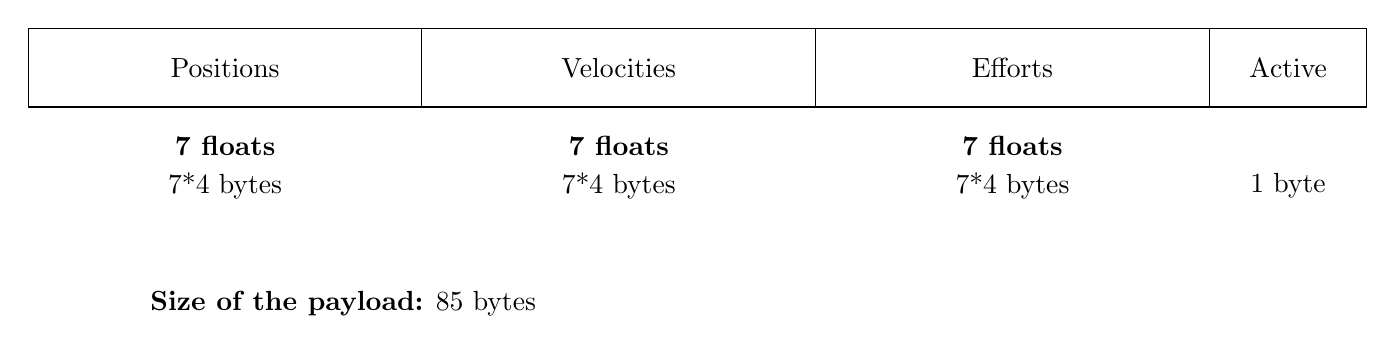
\begin{tikzpicture}

\draw (0,0) rectangle (17,1);
\draw (0,0) rectangle (5,1);
\draw (0,0) rectangle (10,1);
\draw (0,0) rectangle (15,1);

\node at (2.5,0.5) {Positions};
\node at (7.5,0.5) {Velocities};
\node at (12.5,0.5) {Efforts};
\node at (16,0.5) {Active};

\node at (2.5,-0.5) {\textbf{7 floats}};
\node at (7.5,-0.5) {\textbf{7 floats}};
\node at (12.5,-0.5) {\textbf{7 floats}};
%\node at (16,-0.5) {\textbf{n booleans}};

\node at (2.5,-1) {7*4 bytes};
\node at (7.5,-1) {7*4 bytes};
\node at (12.5,-1) {7*4 bytes};
\node at (16,-1) {1 byte};

\node at (4,-2.5) {\textbf{Size of the payload:} 85 bytes}; %I have no idea why i need to put 4 as a coordinate for it to not mess up the rest of the figure
\end{tikzpicture}
\caption{Packet from the sbRIO to ROS for one arm}
\label{received_packet}
\end{figure}

\begin{figure}[H]
\centering
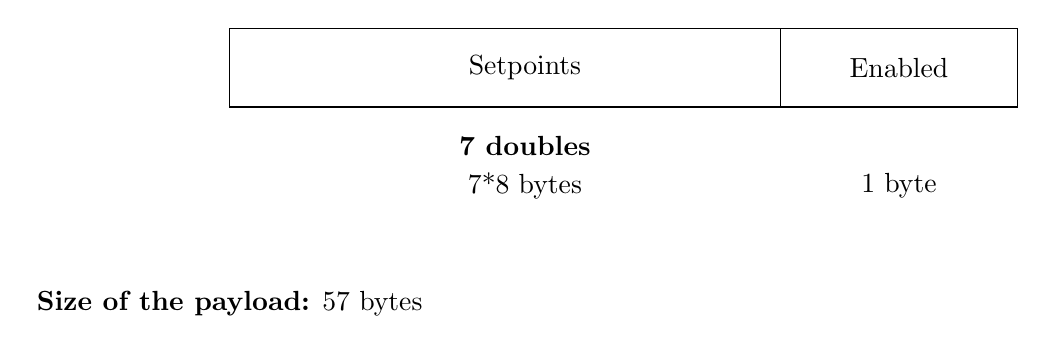
\begin{tikzpicture}

\draw (0,0) rectangle (10,1);
\draw (0,0) rectangle (7,1);

\node at (3.75,0.5) {Setpoints};
\node at (8.5,0.5) {Enabled};

\node at (3.75,-0.5) {\textbf{7 doubles}};
%\node at (8.5,-0.5) {\textbf{n booleans}};

\node at (3.75,-1) {7*8 bytes};
\node at (8.5,-1) {1 byte};

\node at (0,-2.5) {\textbf{Size of the payload:} 57 bytes}; 
\end{tikzpicture}
\caption{Packet from ROS to the sbRIO for one arm}
\label{sent_packet}
\end{figure}

\section{Implementation}
Those improvements need to be implemented on both ROS's and sbRIO's side

\subsection{ROS side}

In order to implement in ROS the improvements described to increase the speed of the communication it is necessary for us to write a new driver. As previously explained, the new driver should use UDP instead of TCP/IP. It should also transmit the actual data without using a \gls{JSON} Stream so that the size of each packets is reduced. In addition to those objectives we would like to modify as little as possible the current structure of the ROS node so that we don't have to rewrite the entire system. 
We just defined three goals that need to be fulfilled when writing the new driver. Let's identify those goals with numbers:
\begin{enumerate}
	\item Replace TCP by UDP
	\item Replace the \gls{JSON} Stream by the numerical values
	\item Modify as little as possible the original driver
\end{enumerate}

The modifications that need to be made in order to carry duty 1. and 2. are related to the communication protocol and the format of the transmitted data which are both handled by the low level driver. In order to fulfill goal 3. we should aim to modify the low level driver only without having consequences on the higher level drivers. This means that the public functions should keep the same prototype and that the format of the data available for them should stay the same (i.e vectors of double)\todo{is it possible to read the mode of the motor driver from the RIO}. We should also try to keep using the boost library used in the original driver to handle threads and mutexes.

The socket initialization for the UDP protocol is very close to the one made for TCP protocol, thanks to this the establishment of the communication with the sbRIO is similar in both the old and new drivers. However, the UDP being connectionless it is not possible to use the same method as before to read incoming data, i.e it is not possible to look if some new data arrived, with UDP it is necessary to constantly be listening for new incoming data. That is why we need to modify the communication loop so that it is always waiting to receive a packet and that it sends data when required. However, if we used the communication loop shown in \figref{original_driver}, the loop would be blocking if no packet was received. To solve this issue we create a new thread that will wait to receive a packet, handle the packet and start again. The new communication structure is shown in \figref{new_driver}.

As explained before, when the \gls{JSON} Stream was removed we decided that we would only send numerical data. And as we keep goal 3. in mind, we need to receive the position, velocity and effort as float and one boolean for each motor and to send a setpoint as a double and a boolean for each motor. The received values must be made available as double for the higher levels by storing them in the vector of doubles. For simplicity we decided that the packet should be following the structure described in \figref{received_packet}. To reach the desired vectors, the received bitcode stored in an array of char is copied in a float variable that we convert in a double and then the value in the vector is updated using this double.

The structure of the sent packet is shown in~\figref{sent_packet}. To build the packet, the same logic as before is used. The bitcode of the numerical values is copied into an array and the array is sent.
In regards to the boolean values, we store them in a byte with 1 bit per value which is possible only because the number of motors for one arm cannot go above 7.

\begin{figure}[H]
\centering
\begin{tikzpicture}

\node[box] (Initialization) at (4,0) {Initialization};
\node[box] (Receive) at ($(4,-3)+(Initialization)$) {Wait to receive\\a packet};
\node[box] (Update_State1) at ($(0,-3)+(Receive)$) {Convert the bitcode};
\node[box] (Update_State2) at ($(0,-3)+(Update_State1)$) {Make the data available for\\higher level processes};

\node[box] (Check) at ($(-4,-3)+(Initialization)$) {Check if there is\\a new control signal};
\node[box] (Send) at ($(0,-3)+(Check)$) {Send};
\node[box] (Sleep) at ($(0,-3)+(Send)$) {Sleep};


\draw[->, ultra thick] (Initialization.south) -- ++(0,-0.5) -|  (Receive.north);
\draw[->, ultra thick] (Receive) -- (Update_State1);
\draw[->, ultra thick] (Update_State1) -- (Update_State2);
\draw[->, ultra thick] (Update_State2.west) -| ++(-1,0) |- (Receive);

\draw[->, ultra thick] (Initialization.south) -- ++(0,-0.5) -| (Check);
\draw[->, ultra thick] (Check) -- (Send);
\draw[->, ultra thick] (Check.east) -| ++(0.5,0) |- (Sleep);%($(0,1.5)+(Sleep)$);
\draw[->, ultra thick] (Send) -- (Sleep);
\draw[->, ultra thick] (Sleep.west) -| ++(-1.5,0) |- (Check);

\node at ($(0,2.1)+(Check)$) {\textbf{thread1}};
\node at ($(0,2.1)+(Receive)$) {\textbf{thread2}};

\node at ($(2.1,0.2)+(Check)$) {No};
\node at ($(0.4,-1)+(Check)$) {Yes};

\end{tikzpicture}
\caption{Structure of the new sbRIO driver}
\label{new_driver}
\end{figure}
\todo{We still need to define the initialization protocol and the packet loss handling}

The driver described is functional, however there is one feature of the TCP/IP that was usefull to our system and that we lost by switching to UDP: the connection timeout detection. As safety is essential in this system, it is necessary to implement an additional layer to the communication to make it more reliable. To implement this safety we have two options: using a free library or implement our own safety protocol. The free librairies that can be found include UDT\cite{UDT}\todo{the author doesn't give his real name, is that ok?} and ENet\cite{ENet}. Those librairies provide a reliable option for long distances communication by adding a number of features. However on the ROS side, it is only necessary to alarm the user of the connection timeout. For such a simple purpose, the free librairies would add to many features that are useless for us and thus slow down the communication. That is why we chose to implement our own safety protocol.


 In order to do so, we decided to add a counter to the current driver. Everytime the thread1 check if some data should be sent, the counter is increased by one. And everytime a packet is received, the counter is reset to 0. In addition to incrementing the counter the thread1 will test the value, if it is superior to 10 (arbitrary value), a message is sent to indicate the packet loss. If the value is superior to 20, a message is sent to indicate connection timeout and the system on ROS is shut down. The new code structure is shown in ~\figref{new_safe_driver}

\begin{figure}[H]
\centering
\begin{tikzpicture}

\node[box] (Initialization) at (4,0) {Initialization};
\node[box] (Receive) at ($(4,-3)+(Initialization)$) {Wait to receive\\a packet};
\node[box] (Reset_Counter) at ($(0,-3)+(Receive)$) {Reset the counter};
\node[box] (Update_State1) at ($(0,-3)+(Reset_Counter)$) {Convert the bitcode};
\node[box] (Update_State2) at ($(0,-3)+(Update_State1)$) {Make the data available for\\higher level processes};

\node[box] (Check) at ($(-4,-3)+(Initialization)$) {Check if there is\\a new control signal};
\node[box] (Send) at ($(0,-2.5)+(Check)$) {Send};
\node[box] (Increment) at ($(0,-2.5)+(Send)$) {Increment the counter};
\node[box] (Connection_Timeout) at ($(0,-2.5)+(Increment)$) {if counter > 10\\throw an error};
\node[box] (Sleep) at ($(0,-2.5)+(Connection_Timeout)$) {Sleep};


\draw[->, ultra thick] (Initialization.south) -- ++(0,-0.5) -|  (Receive.north);
\draw[->, ultra thick] (Receive) -- (Reset_Counter);
\draw[->, ultra thick] (Reset_Counter) -- (Update_State1);
\draw[->, ultra thick] (Update_State1) -- (Update_State2);
\draw[->, ultra thick] (Update_State2.west) -| ++(-1,0) |- (Receive);

\draw[->, ultra thick] (Initialization.south) -- ++(0,-0.5) -| (Check);
\draw[->, ultra thick] (Check) -- (Send);
\draw[->, ultra thick] (Check.east) -| ++(0.75,0) |- (Increment);%($(0,1.5)+(Sleep)$);
\draw[->, ultra thick] (Send) -- (Increment);
\draw[->, ultra thick] (Increment) -- (Connection_Timeout);
\draw[->, ultra thick] (Connection_Timeout) -- (Sleep);
\draw[->, ultra thick] (Sleep.west) -| ++(-1.5,0) |- (Check);

\node at ($(0,2.1)+(Check)$) {\textbf{thread1}};
\node at ($(0,2.1)+(Receive)$) {\textbf{thread2}};

\node at ($(2.1,0.2)+(Check)$) {No};
\node at ($(0.4,-1)+(Check)$) {Yes};

\end{tikzpicture}
\caption{Structure of the new sbRIO driver with connection timeout detection}
\label{new_safe_driver}
\end{figure}

\subsection{sbRIO side}

connecting some boxes

\section{Measurements}

1.5m above the ground

Measurements of the delays in the system before and after "improvements"